\documentclass{article}

% \documentclass[preview]{standalone}
% If the image is too large to fit on this documentclass use
% img_width = 2, img_depth = 2
% instead and customize the height and width (in cm) to fit.
% Large images may run out of memory quickly.
% To fix this use the LuaLaTeX compiler, which dynamically
% allocates memory.
\usepackage[braket, qm]{qcircuit}
\usepackage{amsmath}
\pdfmapfile{+sansmathaccent.map}
% \usepackage[landscape]{geometry}
% Comment out the above line if using the beamer documentclass.


\title{Visualizing the Quantum Fourier Transform in Qiskit}
\subtitle{A Short Introduction to Both}
\usepackage{pythontex}
\usepackage{url}

\begin{document}

\begin{center}
    
    The QFT generalizes the discrete Fourier transform via: 
    \[
    \vert j \rangle  \rightarrow  \frac{1}{\sqrt{N}} \sum_{k=0}^{N-1} e^{2\pi ijk/N} \vert k \rangle   
    \]. 
   
    Which is unitary, and so atleast has some quantum circuit approximating it. 



\end{center}     
       
Examples:

The QFT for the 1-qubit case should look familiar:

\[ \frac{1}{\sqrt{2}} 
\begin{bmatrix}
    1 & 1 \\
    1 & -1\\
\end{bmatrix}
\]. 

      
So we already have some gate for this:

\begin{equation*}
    \Qcircuit @C=1.0em @R=0.2em @!R {
	 	\lstick{ {q}_{0} :  } & \gate{\mathrm{H}} & \qw & \qw\\
	 	 }
\end{equation*}



      
    \end{center}
\end{frame}    

\begin{frame}
    \frametitle{2-qubit QFT}
    \begin{center}
       In the computational basis, the QFT for two qubits takes the form:

\medskip

\medskip

       $ \frac{1}{2} 
      \begin{bmatrix}
           1 & 1 & 1 & 1 \\
           1 & i & -1 &-i \\
           1 & -1 & 1 & -1\\
           1 & -i & -1& i\\
       \end{bmatrix}$

       \vspace{.61cm}

       And is represented by the circuit:

\vspace{-.26cm}

\begin{equation*}
    \Qcircuit @C=1.0em @R=0.2em @!R {
        \lstick{ {q}_{0} :  } & \gate{\mathrm{H}} & \ctrl{1} & \dstick{\hspace{2.3em}\mathrm{CP}\,\mathrm{(}\mathrm{\pi / 2}\mathrm{)}} \qw &\qw &\qw & \qw & \qw & \qswap & \qw & \qw\\
        \lstick{ {q}_{1} :  } & \qw & \control \qw & \qw & \qw & \qw &\qw & \gate{\mathrm{H}} & \qswap \qwx[-1] & \qw & \qw\\
	 }
\end{equation*} where 
$CP\left( \theta  \right) =\begin{bmatrix}
    1 & 0  &0&0\\
    0&1&0&0\\
    0&0&1&0\\
    0&0&0&e^{{i\theta }} 
\end{bmatrix}$





    \end{center}


For your consideration,

\begin{equation*}
    \Qcircuit @C=1.0em @R=0.2em @!R {
        \lstick{ {q}_{0} :  } & \gate{\mathrm{H}} & \ctrl{1} & \dstick{\hspace{2.3em}\mathrm{CP}\,\mathrm{(}\mathrm{\pi / 2}\mathrm{)}} \qw &\qw &\qw & \qw & \qw & \qswap & \qw & \qw\\
        \lstick{ {q}_{1} :  } & \qw & \control \qw & \qw & \qw & \qw &\qw & \gate{\mathrm{H}} & \qswap \qwx[-1] & \qw & \qw\\
	 }
\end{equation*} 

\vspace{.5cm}

\begin{center}

\hbox{
$\begin{bmatrix}
    1 & 0  &0&0\\
    0&0&1&0\\
    0&1&0&0\\
    0&0&0&1 
\end{bmatrix}
\begin{bmatrix}
    1 & 1  &0&0\\
    1&-1&0&0\\
    0&0&1&1\\
    0&0&1&-1
\end{bmatrix}
\begin{bmatrix}
    1 & 0  &0&0\\
    0&1&0&0\\
    0&0&1&0\\
    0&0&0&e^{i\pi /2 } 
\end{bmatrix}
\begin{bmatrix}
    1 & 0  &1&0\\
    0& 1&0&1\\
    1&0&-1&0\\
    0&1&0&-1
\end{bmatrix}



$}
   
= $\begin{bmatrix}
           1 & 1 & 1 & 1 \\
           1 & i & -1 &-i \\
           1 & -1 & 1 & -1\\
           1 & -i & -1& i\\
       \end{bmatrix}$
 
\end{center}



    \begin{center}
    
Written out in terms of the $8$th roots of unity, the matrix form of the 3 qubit QFT is:


\[ \frac{1}{2\sqrt{2}} 
\begin{bmatrix}
    1 & 1 & 1 & 1 & 1 & 1 & 1 & 1\\
    1 & \omega &\omega ^2      &\omega ^3  &\omega ^{4} &\omega ^{5} &\omega ^{6} &\omega ^{7}\\
    1 & \omega ^2&\omega ^{4}  &\omega^{6} &1       &\omega ^2&\omega ^{4} &\omega ^{6}\\
    1 &\omega ^{3}&\omega ^{6} &\omega     &\omega ^{4} &\omega ^{7} &\omega ^2&\omega ^{5} \\
    1 &\omega ^{4}&           1&\omega^{4} &1&\omega ^{4} &1 & \omega ^{4}   \\
    1 &\omega ^{5}&\omega ^{2} &\omega^{7} &\omega ^{4} &\omega &\omega ^6&\omega ^{3} \\
    1 &\omega ^{6}&\omega ^{4} &\omega^2  &1&\omega ^{6} &\omega ^4&\omega ^{2} \\
    1 &\omega ^{7}&\omega ^{6} &\omega^{5}  &\omega ^{4} &\omega ^{3} &\omega ^2&\omega  \\
\end{bmatrix}
\]. 

    \end{center}



With a circuit diagram:

\begin{equation*}    \Qcircuit @C=1.0em @R=0.2em @!R { \lstick{ {q}_{0} :  } & \qw & \qw & \qw & \qw & \qw & \control \qw & \qw & \qw & \qw & \qw & \control \qw & \dstick{\hspace{2.0em}\mathrm{CP}\mathrm{(}\mathrm{\pi /2}\mathrm{)}} \qw & \qw & \qw & \gate{\mathrm{H}} & \qswap & \qw & \qw \\
\lstick{ {q}_{1} :  } & \qw & \control \qw & \dstick{\hspace{2.0em}\mathrm{CP}\,\mathrm{(}\mathrm{\pi / 2}\mathrm{)}} \qw & \qw & \qw & \qw & \dstick{\hspace{2.0em}\mathrm{CP}\mathrm{(}\mathrm{\pi / 4}\mathrm{)}} \qw & \qw & \qw & \gate{\mathrm{H}} & \ctrl{-1} & \qw & \qw & \qw & \qw & \qw & \qw & \qw \\
\lstick{ {q}_{2} :  } & \gate{\mathrm{H}} & \ctrl{-1} & \qw & \qw & \qw & \ctrl{-2} & \qw & \qw & \qw & \qw & \qw & \qw & \qw & \qw & \qw & \qswap \qwx[-2] & \qw & \qw }\end{equation*}

Let's see what it does to some qubits on the bloch sphere:

\begin{pyblock}
from qiskit.circuit.library import QFT
qft = QFT(3)
qft3_000 = execute(qft, backend).result()
plot_bloch_multivector(qft3_000.get_statevector())
\end{pyblock}

\begin{center}
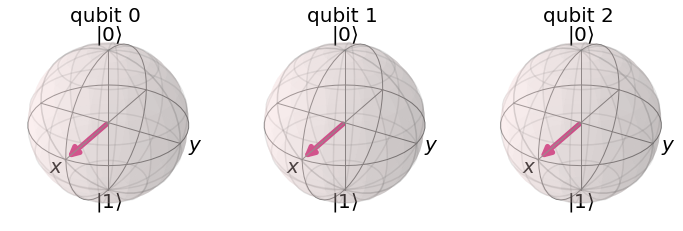
\includegraphics[scale=.25]{Downloads/q000.png}
\end{center}


\begin{pyblock}
plot_bloch_multivector(qft3_001.get_statevector())
\end{pyblock}

\begin{center}
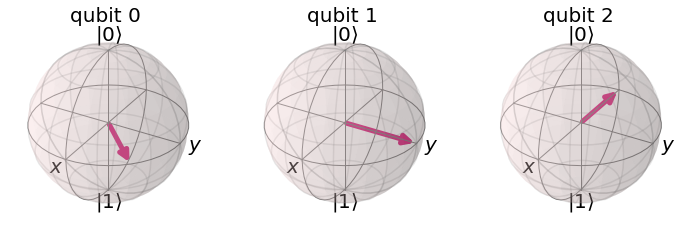
\includegraphics[scale=.25]{Downloads/q001.png}
\end{center}

\begin{pyblock}
plot_bloch_multivector(qft3_010.get_statevector())
\end{pyblock}

\begin{center}
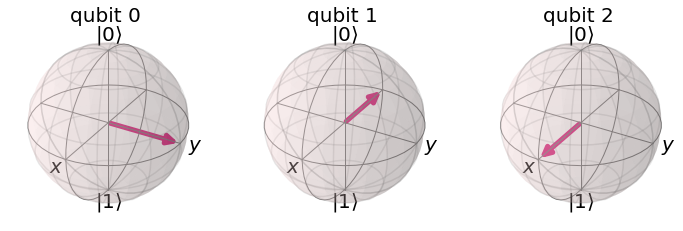
\includegraphics[scale=.25]{Downloads/q010.png}
\end{center}

\begin{pyblock}
plot_bloch_multivector(qft3_011.get_statevector())
\end{pyblock}

\begin{center}
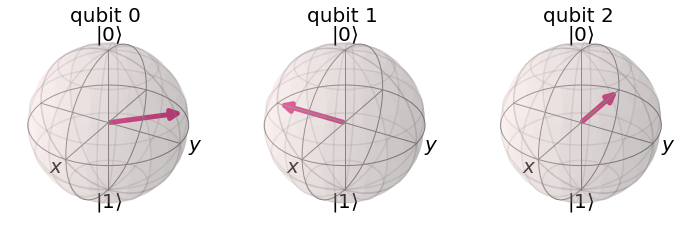
\includegraphics[scale=.25]{Downloads/q011.png}
\end{center}



   
    This relative rotation of the output bits by some angle $\theta ^{2n} $ hints at the identity proven in \cite{NC},
    where $0.b_1..b_n=b_1/2+... + b_n/2^{n} $ 
\medskip

    $
        \vert j_1,...,j_n \rangle  =  
    $
    \hspace{-.9cm} \[
        \frac{\left( \vert 0 \rangle  + e^{2\pi i_0.j_n} \vert 1 \rangle  \right)\otimes \left( \left( \vert 0 \rangle  + e^{2\pi i_0.j_{n-1}j_n} \vert 1 \rangle \right)\otimes ...\otimes \left( \vert 0 \rangle  + e^{2\pi i_0.j_1...j_n}  \vert 1 \rangle  \right)  }{2^{n/2} } 
    \]. 
    

    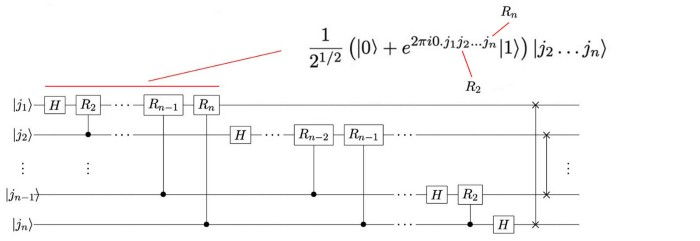
\includegraphics[scale=.5]{Downloads/nqbqft.jpeg}\cite{nqbqft}


\bibliographystyle{plain}
\bibliography{quantum.bib}


\end{document}
